% $Id: template.tex 11 2007-04-03 22:25:53Z jpeltier $

\documentclass{vgtc}                          % final (conference style)
%\documentclass[review]{vgtc}                 % review
%\documentclass[widereview]{vgtc}             % wide-spaced review
%\documentclass[preprint]{vgtc}               % preprint
%\documentclass[electronic]{vgtc}             % electronic version

\let\ifpdf\relax

%% Uncomment one of the lines above depending on where your paper is
%% in the conference process. ``review'' and ``widereview'' are for review
%% submission, ``preprint'' is for pre-publication, and the final version
%% doesn't use a specific qualifier. Further, ``electronic'' includes
%% hyperreferences for more convenient online viewing.

%% Please use one of the ``review'' options in combination with the
%% assigned online id (see below) ONLY if your paper uses a double blind
%% review process. Some conferences, like IEEE Vis and InfoVis, have NOT
%% in the past.

%% Figures should be in CMYK or Grey scale format, otherwise, colour 
%% shifting may occur during the printing process.

%% These three lines bring in essential packages: ``mathptmx'' for Type 1 
%% typefaces, ``graphicx'' for inclusion of EPS figures. and ``times''
%% for proper handling of the times font family.

\usepackage{mathptmx}
\usepackage{graphicx}
\usepackage{times}
\usepackage{url}

%% We encourage the use of mathptmx for consistent usage of times font
%% throughout the proceedings. However, if you encounter conflicts
%% with other math-related packages, you may want to disable it.

%% If you are submitting a paper to a conference for review with a double
%% blind reviewing process, please replace the value ``0'' below with your
%% OnlineID. Otherwise, you may safely leave it at ``0''.
\onlineid{0}

%% declare the category of your paper, only shown in review mode
\vgtccategory{Research}

%% allow for this line if you want the electronic option to work properly
\vgtcinsertpkg

%% In preprint mode you may define your own headline.
%\preprinttext{To appear in an IEEE VGTC sponsored conference.}

%% Paper title.

\title{Interactive Visual Analytics of Molecular Data in Immersive Environments via a Semantic Definition of the Content and the Context}

%% This is how authors are specified in the conference style

%% Author and Affiliation (single author).
%%\author{Roy G. Biv\thanks{e-mail: roy.g.biv@aol.com}}
%%\affiliation{\scriptsize Allied Widgets Research}

%% Author and Affiliation (multiple authors with single affiliations).
%%\author{Roy G. Biv\thanks{e-mail: roy.g.biv@aol.com} %
%%\and Ed Grimley\thanks{e-mail:ed.grimley@aol.com} %
%%\and Martha Stewart\thanks{e-mail:martha.stewart@marthastewart.com}}
%%\affiliation{\scriptsize Martha Stewart Enterprises \\ Microsoft Research}

%% Author and Affiliation (multiple authors with multiple affiliations)
\author{Mikael Trellet\thanks{e-mail: trellet@limsi.fr}\\ %
      \parbox{1.4in}{\scriptsize \centering Venise group \\ LIMSI-CNRS }%
\and Nicolas Férey\thanks{e-mail: ferey@limsi.fr}\\ %
     \parbox{1.4in}{\scriptsize \centering Venise group \\ LIMSI-CNRS }%
\and Marc Baaden\thanks{e-mail: baaden@smplinux.de}\\ %
     \parbox{1.4in}{\scriptsize \centering LBT \\ IBPC-CNRS}
\and Patrick Bourdot\thanks{e-mail: bourdot@limsi.fr}\\ %
     \parbox{1.4in}{\scriptsize \centering Venise group \\ LIMSI-CNRS }}%

%% A teaser figure can be included as follows, but is not recommended since
%% the space is now taken up by a full width abstract.
%\teaser{
%  \includegraphics[width=1.5in]{sample.eps}
%  \caption{Lookit! Lookit!}
%}

%% Abstract section.
\abstract{
Bringing together, in a unique immersive environment, visualisation and analysis of scientific and complex data requires a thorough approach in order to fulfill scientists specific expectations. This approach needs to consider both the highly heterogeneous nature of data, the dynamic interactions between the experts and the data as well as the large amount of data involved today in a scientific study.
Whereas small and static scientific datasets can be quickly deciphered thanks to standard immersive tools such as 3D visualisation softwares, bigger and dynamic datasets overcome the analytical capacity of these tools and requires an efficient platform to manipulate the data they expose. We raise through the example of the structural biology field the need for an approach based on a high-level definition of the content (scientific data) and the context (immersive environments and interfaces) in order to setup a platform able to present to the user a dynamic and intelligent representation of his data and to provide direct ways to interact with them. This approach is based on the semantic definition of all the concepts, abstract and concrete, manipulated in the environments which allows for an adaptive and interactive experience of both visualisation and analysis.
} % end of abstract

%% ACM Computing Classification System (CCS). 
%% See <http://www.acm.org/class/1998/> for details.
%% The ``\CCScat'' command takes four arguments.

\CCScatlist{ 
  \CCScat{K.6.1}{Management of Computing and Information Systems}%
{Project and People Management}{Life Cycle};
  \CCScat{K.7.m}{The Computing Profession}{Miscellaneous}{Ethics}
}

%% Copyright space is enabled by default as required by guidelines.
%% It is disabled by the 'review' option or via the following command:
% \nocopyrightspace

%%%%%%%%%%%%%%%%%%%%%%%%%%%%%%%%%%%%%%%%%%%%%%%%%%%%%%%%%%%%%%%%
%%%%%%%%%%%%%%%%%%%%%% START OF THE PAPER %%%%%%%%%%%%%%%%%%%%%%
%%%%%%%%%%%%%%%%%%%%%%%%%%%%%%%%%%%%%%%%%%%%%%%%%%%%%%%%%%%%%%%%%

\begin{document}

%% The ``\maketitle'' command must be the first command after the
%% ``\begin{document}'' command. It prepares and prints the title block.

%% the only exception to this rule is the \firstsection command
\firstsection{Introduction}

\maketitle

%% \section{Introduction} 


With the increasing amount of scientific data that experts have to manipulate, the need for platforms able to handle the data flow complexity is strong. It is particularly true in structural biology where the simulation processes can now deal with very large and heterogeneous molecular structures. These structures can be composed of several millions of particles and consist of the molecule as well as its environment, adding to the complexity and the need to go beyond standard visualisation solutions.
Then, the amount and complexity available to structural biology experts force them to move towards integrated systems where visualisation and analysis can be merged together. These integrated systems have to be able to mix heterogeneous data by presenting them in the same working space and let the user interact with them in the most direct way possible. Immersive environments address these two requirements by providing both a large and putatively infinite virtual scene to display the data as well as a direct approach to explore and manipulate them.


However, today, most of platforms used by the experts in structural biology compartmentalize the visualisation of data and their analysis into two different and independent processes based on different tools.
The explanation of this splitting is the significant differences between the data handled by the 3D visualisation softwares and the analytical tools.
On one side, 3D visualisation solutions explore and manipulate 3D structures coordinates composing the molecular complex that will be displayed. The scene seen by the user will be composed of 3D objects reporting the overall shape of a particular molecule and its environment at a particular state. This scene can be static if we are interested in only one state of the molecule but it is often dynamic with a whole simulated trajectory of the molecule undergoing some energetic constraints coming from a physical simulation program.
Analysis tools, on the other side, take into input raw number, on various format and from various sources depending on the pipeline in which they are used. Their outputs are graphical representation of trends or comparisons between elements parameters in a way that experts can quickly understand and use these information to guide their next hypotheses.
During the process that tries to decipher a scientific mechanism, and as we highlighted previously, experts constantly move from visualisation tools to analysis tools and vice versa, wasting a precious time along the way.

A scenario where the 3D visualisation of a molecular event would be coupled to a monitoring of the properties evolution, sub-elements distance variations and simulation parameters progression into a single working environment where the user would see any action performed in one space (either 3D visualisation or analysis) has a coherent graphical impact on the second space to filter or highlight the parameter or sub-ensemble of objects targeted by the expert appear as a major improvement of today available tools.

Immersive environments favor the combination of components and provide several ways to merge 
data and processes coming from different sources for a particular task. But this combination of heterogeneous information brings several issues that need to be tackled in order to propose a fully-functional immersive environments where scientists will have the possibility to visualise, analyse and interact with their data.

One of the first issue is the lack of actual platform in structural biology able to gather at the same place information dedicated either for visualisation purposes or for analyses purposes. This link between these two worlds would bring the possibility for the scientists to manipulate raw data superimposed on their 3D models of molecules and then add a much better way of deciphering a particular molecular mechanism.
We believe that the setup of a database with a high-level representation of all the data leads to an efficient way to mix visualisation and analysis. By ordering knowledge, it is possible to create direct links between individuals and properties and then setup automatic retrievals of data each time an expert would need it.
Another aspect to consider for an immersive platform combining visualisation and analysis is the interaction between the experts and the ensemble of data that will be at his disposal.

The semantic definition of the applicative field can be enough to implement dynamic links between visual and analytical properties but do not allow for a specific way to interact with the data. As a result, we extended the definition of the structural biology content to the immersive context in which the platform will be used.
By doing so, we are able to combine information from both the expert knowledge and the user context in order to define intelligent interactions during the immersive working session.


, like the pore opening of a large protein buried in a cell membrane to allow water molecules to reach the inner and outer part of a cell, 

\section{Semantic definition of the platform}

In Computer Sciences, the knowledge representation is often associated to the notion of ontology. An ontology is defined as a structured and hierarchical ensemble of concepts and relationships allowing to define part or a whole field. An ontology must be understandable both by the computer systems and by the humans. It has indeed to be integrated in computing processes and to be setup by experts of a field.

Ontologies must allow the classification of any specific value or information into a pre-defined schema as instances of elements of this schema. For instance, a very simple ontology consisting of the two concepts "Atom" and "Charge" linked by a possessive relationship as illustrated on the figure \ref{simple_ontology}.
If any atom is added to a database defined by this ontology, an instance of the concept "Atom" will be created and a value of charge will be added to the property "Charge". The atom and the value will be linked and it will be possible to access them by searching either for the instance or for the property.

\subsection{Formalism choice}

The setup of ontologies in order to standardized knowledge in scientific fields has undergone an important and spontaneous growth at the end of the 90s~\cite{schulze-kremer_ontologies_2002, baker_ontology_1999}.

Several formalisms exist to create ontologies and use them to define databases. We chose to use the Web Semantic approach in order to setup our own ontology. 
The Web Semantic has been created by the \textit{World Wide Web Consortium} under the lead of Tim Berners-Lee, with the aim to share semantic data on the web. It is broadly used by the biggest web companies to uniformly store and share data. It belongs the family of the description logics that uses the notions of \textit{concepts, roles} and \textit{individuals}. The \textit{concepts} are the sub-ensemble of elements in a specific universe, the \textit{roles} are the links between the elements and the \textit{individuals} are the elements of the universe~\cite{}. In our previous example, "Atom" and "Charge" would be \textit{concepts}, "has-a" a \textit{role} and the oxygen an \textit{individual}, as an instance of the \textit{concept} "Atom".
Each layer of the Web Semantics (ontology, experimental data, querying process, etc.) has been associated to a language or a format. The different layers and their associated formats are described in the figure~\ref{web_semantic_hierarchy}. 

\begin{figure}[htb]
  \centering
  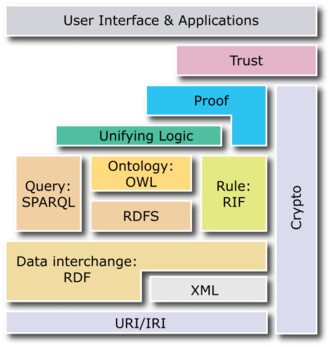
\includegraphics[width=.5\linewidth]{figures/web_semantic_hierarchy.png}
  \caption{Hierarchical schema of the Web Semantics multiple layer architecture}
  \label{web_semantic_hierarchy}
\end{figure}

Bioinformatics, tightly anchored with structural biology, uses ontology for a long time. The most significant example is the genomic field where data flow quickly became unable to handle without a proper and standard organization of the data~\cite{schuurman}. \textit{Gene Ontology}~\cite{ashburner} was then created to group genomic data into a uniform format and databse and is now one of the most cited ontology. Several biological databases or organizations like UniProtKB\footnote{\url{http://www.uniprot.org/uniprot/}} or the \textit{Open Biomedical Ontologies}~\cite{}, provide ways to access data or ontologies under RDF or OWL format to allow their use in expert tools or specific pipelines.

\section{Exposition}

Lorem ipsum dolor sit amet, consetetur sadipscing elitr, sed diam
nonumy eirmod tempor invidunt ut labore et dolore magna aliquyam erat,
sed diam voluptua. At vero eos et accusam et justo duo dolores et ea
rebum. Stet clita kasd gubergren, no sea takimata sanctus est Lorem
ipsum dolor sit amet. Lorem ipsum dolor sit amet, consetetur
sadipscing elitr, sed diam nonumy eirmod tempor invidunt ut labore et
dolore magna aliquyam erat, sed diam voluptua. At vero eos et accusam
et justo duo dolores et ea rebum. Stet clita kasd gubergren, no sea
takimata sanctus est Lorem ipsum dolor sit amet. Lorem ipsum dolor sit
amet, consetetur sadipscing elitr, sed diam nonumy eirmod tempor
invidunt ut labore et dolore magna aliquyam erat, sed diam
voluptua. At vero eos et accusam et justo duo dolores et ea
rebum~\cite{ware:2004:IVP}. Stet clita kasd gubergren, no sea takimata
sanctus est Lorem ipsum dolor sit amet.

Duis autem vel eum iriure dolor in hendrerit in vulputate velit esse
molestie consequat, vel illum dolore eu feugiat nulla facilisis at
vero eros et accumsan et iusto odio dignissim qui blandit praesent
luptatum zzril delenit augue duis dolore te feugait nulla
facilisi. Lorem ipsum dolor sit amet, consectetuer adipiscing elit,
sed diam nonummy nibh euismod tincidunt ut laoreet dolore magna
aliquam erat volutpat~\cite{kindlmann:1999:SAG}.

Ut wisi enim ad minim veniam, quis nostrud exerci tation ullamcorper
suscipit lobortis nisl ut aliquip ex ea commodo
consequat~\cite{levoy:1989:DSV}. Duis autem vel eum iriure dolor in
hendrerit in vulputate velit esse molestie consequat, vel illum dolore
eu feugiat nulla facilisis at vero eros et accumsan et iusto odio
dignissim qui blandit praesent luptatum zzril delenit augue duis
dolore te feugait nulla facilisi.

Lorem ipsum dolor sit amet, consetetur sadipscing elitr, sed diam
nonumy eirmod tempor invidunt ut labore et dolore magna aliquyam erat,
sed diam voluptua. At vero eos et accusam et justo duo dolores et ea
rebum. Stet clita kasd gubergren, no sea takimata sanctus est Lorem
ipsum dolor sit amet. Lorem ipsum dolor sit amet, consetetur
sadipscing elitr, sed diam nonumy eirmod tempor invidunt ut labore et
dolore magna aliquyam erat, sed diam voluptua. At vero eos et accusam
et justo duo dolores et ea rebum. Stet clita kasd gubergren, no sea
takimata sanctus est Lorem ipsum dolor sit amet. Lorem ipsum dolor sit
amet, consetetur sadipscing elitr, sed diam nonumy eirmod tempor
invidunt ut labore et dolore magna aliquyam erat, sed diam
voluptua. At vero eos et accusam et justo duo dolores et ea
rebum. Stet clita kasd gubergren, no sea takimata sanctus est Lorem
ipsum dolor sit amet.

Lorem ipsum dolor sit amet, consetetur sadipscing elitr, sed diam
nonumy eirmod tempor invidunt ut labore et dolore magna aliquyam erat,
sed diam voluptua. At vero eos et accusam et justo duo dolores et ea
rebum. Stet clita kasd gubergren, no sea takimata sanctus est Lorem
ipsum dolor sit amet. Lorem ipsum dolor sit amet, consetetur
sadipscing elitr, sed diam nonumy eirmod tempor invidunt ut labore et
dolore magna aliquyam erat, sed diam voluptua. At vero eos et accusam
et justo duo dolores et ea rebum. Stet clita kasd gubergren, no sea
takimata sanctus est Lorem ipsum dolor sit amet. Lorem ipsum dolor sit
amet, consetetur sadipscing elitr, sed diam nonumy eirmod tempor
invidunt ut labore et dolore magna aliquyam erat, sed diam
voluptua. At vero eos et accusam et justo duo dolores et ea
rebum. Stet clita kasd gubergren, no sea takimata sanctus est Lorem
ipsum dolor sit amet.

Lorem ipsum dolor sit amet, consetetur sadipscing elitr, sed diam
nonumy eirmod tempor invidunt ut labore et dolore magna aliquyam erat,
sed diam voluptua. At vero eos et accusam et justo duo dolores et ea
rebum. Stet clita kasd gubergren, no sea takimata sanctus est Lorem
ipsum dolor sit amet. Lorem ipsum dolor sit amet, consetetur
sadipscing elitr, sed diam nonumy eirmod tempor invidunt ut labore et
dolore magna aliquyam erat, sed diam voluptua.

\begin{equation}
 \sum_{j=1}^{z} j = \frac{z(z+1)}{2}
\end{equation}

Lorem ipsum dolor sit amet, consetetur sadipscing elitr, sed diam
nonumy eirmod tempor invidunt ut labore et dolore magna aliquyam erat,
sed diam voluptua. At vero eos et accusam et justo duo dolores et ea
rebum. Stet clita kasd gubergren, no sea takimata sanctus est Lorem
ipsum dolor sit amet. Lorem ipsum dolor sit amet, consetetur
sadipscing elitr, sed diam nonumy eirmod tempor invidunt ut labore et
dolore magna aliquyam erat, sed diam voluptua. At vero eos et accusam
et justo duo dolores et ea rebum. Stet clita kasd gubergren, no sea
takimata sanctus est Lorem ipsum dolor sit amet. Lorem ipsum dolor sit
amet, consetetur sadipscing elitr, sed diam nonumy eirmod tempor
invidunt ut labore et dolore magna aliquyam erat, sed diam
voluptua. At vero eos et accusam et justo duo dolores et ea
rebum. Stet clita kasd gubergren, no sea takimata sanctus est Lorem
ipsum dolor sit amet.

Lorem ipsum dolor sit amet, consetetur sadipscing elitr, sed diam
nonumy eirmod tempor invidunt ut labore et dolore magna aliquyam erat,
sed diam voluptua. At vero eos et accusam et justo duo dolores et ea
rebum. Stet clita kasd gubergren, no sea takimata sanctus est Lorem
ipsum dolor sit amet. Lorem ipsum dolor sit amet, consetetur
sadipscing elitr, sed diam nonumy eirmod tempor invidunt ut labore et
dolore magna aliquyam erat, sed diam voluptua. At vero eos et accusam
et justo duo dolores et ea rebum. Stet clita kasd gubergren, no sea
takimata sanctus est Lorem ipsum dolor sit amet. Lorem ipsum dolor sit
amet, consetetur sadipscing elitr, sed diam nonumy eirmod tempor
invidunt ut labore et dolore magna aliquyam erat, sed diam
voluptua. At vero eos et accusam et justo duo dolores et ea
rebum. Stet clita kasd gubergren, no sea takimata sanctus est Lorem
ipsum dolor sit amet.

Lorem ipsum dolor sit amet, consetetur sadipscing elitr, sed diam
nonumy eirmod tempor invidunt ut labore et dolore magna aliquyam erat,
sed diam voluptua. At vero eos et accusam et justo duo dolores et ea
rebum. Stet clita kasd gubergren, no sea takimata sanctus est Lorem
ipsum dolor sit amet. Lorem ipsum dolor sit amet, consetetur
sadipscing elitr, sed diam nonumy eirmod tempor invidunt ut labore et
dolore magna aliquyam erat, sed diam voluptua. At vero eos et accusam
et justo duo dolores et ea rebum. Stet clita kasd gubergren, no sea
takimata sanctus est Lorem ipsum dolor sit amet. 

Lorem ipsum dolor sit amet, consetetur sadipscing elitr, sed diam
nonumy eirmod tempor invidunt ut labore et dolore magna aliquyam erat,
sed diam voluptua. At vero eos et accusam et justo duo dolores et ea
rebum. Stet clita kasd gubergren, no sea takimata sanctus est Lorem
ipsum dolor sit amet. Lorem ipsum dolor sit amet, consetetur
sadipscing elitr, sed diam nonumy eirmod tempor invidunt ut labore et
dolore magna aliquyam erat, sed diam voluptua. At vero eos et accusam
et justo duo dolores et ea rebum. Stet clita kasd gubergren, no sea
takimata sanctus est Lorem ipsum dolor sit amet. Lorem ipsum dolor sit
amet, consetetur sadipscing elitr, sed diam nonumy eirmod tempor
invidunt ut labore et dolore magna aliquyam erat, sed diam
voluptua. At vero eos et accusam et justo duo dolores et ea
rebum. Stet clita kasd gubergren, no sea takimata sanctus est Lorem
ipsum dolor sit amet.

\begin{table}
  \caption{Vis Paper Acceptance Rate}
  \label{vis_accept}
  \scriptsize
  \begin{center}
    \begin{tabular}{cccc}
      Year & Submitted & Accepted & Accepted (\%)\\
    \hline
      1994 &  91 & 41 & 45.1\\
      1995 & 102 & 41 & 40.2\\
      1996 & 101 & 43 & 42.6\\
      1997 & 117 & 44 & 37.6\\
      1998 & 118 & 50 & 42.4\\
      1999 & 129 & 47 & 36.4\\
      2000 & 151 & 52 & 34.4\\
      2001 & 152 & 51 & 33.6\\
      2002 & 172 & 58 & 33.7\\
      2003 & 192 & 63 & 32.8\\
      2004 & 167 & 46 & 27.6\\
      2005 & 268 & 88 & 32.8\\
      2006 & 228 & 63 & 27.6
    \end{tabular}
  \end{center}
\end{table}

\begin{figure}[htb]
  \centering
  \includegraphics[width=1.5in]{sample.eps}
  \caption{Sample illustration.}
\end{figure}

\subsection{Mezcal Head}

Duis autem~\cite{Lorensen:1987:MCA} vel eum iriure dolor in hendrerit
in vulputate velit esse molestie consequat, vel illum dolore eu
feugiat nulla facilisis at vero eros et accumsan et iusto odio
dignissim qui blandit praesent luptatum zzril delenit augue duis
dolore te feugait nulla facilisi. Lorem ipsum dolor sit amet,
consectetuer adipiscing elit, sed diam nonummy nibh euismod tincidunt
ut laoreet dolore magna aliquam erat volutpat%
\footnote{Footnotes appear at the bottom of the column}.


\subsubsection{Ejector Seat Reservation}

Ut wisi enim ad minim veniam, quis nostrud exerci tation ullamcorper
suscipit lobortis nisl ut aliquip ex ea commodo
consequat~\cite{Nielson:1991:TAD}. Duis autem vel eum iriure dolor in
hendrerit in vulputate velit esse molestie consequat, vel illum dolore
eu feugiat nulla facilisis at vero eros et accumsan et iusto odio
dignissim qui blandit praesent luptatum zzril delenit augue duis
dolore te feugait nulla facilisi.

\paragraph{Rejected Ejector Seat Reservation}

Ut wisi enim ad minim veniam, quis nostrud exerci tation ullamcorper
suscipit lobortis nisl ut aliquip ex ea commodo consequat. Duis autem
vel eum iriure dolor in hendrerit in vulputate velit esse molestie

\section{Conclusion}

Lorem ipsum dolor sit amet, consetetur sadipscing elitr, sed diam
nonumy eirmod tempor invidunt ut labore et dolore magna aliquyam erat,
sed diam voluptua. At vero eos et accusam et justo duo dolores et ea
rebum. Stet clita kasd gubergren, no sea takimata sanctus est Lorem
ipsum dolor sit amet. Lorem ipsum dolor sit amet, consetetur
sadipscing elitr, sed diam nonumy eirmod tempor invidunt ut labore et
dolore magna aliquyam erat, sed diam voluptua. At vero eos et accusam
et justo duo dolores et ea rebum. Stet clita kasd gubergren, no sea
takimata sanctus est Lorem ipsum dolor sit amet. Lorem ipsum dolor sit
amet, consetetur sadipscing elitr, sed diam nonumy eirmod tempor
invidunt ut labore et dolore magna aliquyam erat, sed diam
voluptua. At vero eos et accusam et justo duo dolores et ea
rebum. Stet clita kasd gubergren, no sea takimata sanctus est Lorem
ipsum dolor sit amet.

Lorem ipsum dolor sit amet, consetetur sadipscing elitr, sed diam
nonumy eirmod tempor invidunt ut labore et dolore magna aliquyam erat,
sed diam voluptua. At vero eos et accusam et justo duo dolores et ea
rebum. Stet clita kasd gubergren, no sea takimata sanctus est Lorem
ipsum dolor sit amet. Lorem ipsum dolor sit amet, consetetur
sadipscing elitr, sed diam nonumy eirmod tempor invidunt ut labore et
dolore magna aliquyam erat, sed diam voluptua. At vero eos et accusam
et justo duo dolores et ea rebum. 

%% if specified like this the section will be ommitted in review mode
\acknowledgements{
The authors wish to thank A, B, C. This work was supported in part by
a grant from XYZ.}

\bibliographystyle{abbrv}
%%use following if all content of bibtex file should be shown
%\nocite{*}
\bibliography{virtual_analytics}
\end{document}
